\documentclass[12pt]{article}
\usepackage{graphicx}
\usepackage[margin=30mm, paper = a4paper]{geometry}
\usepackage{minted}
\usepackage{multicol}
\usepackage[english]{babel}

\title{Taking a propositional logic and finding if the logic is tautology or not}
\author{Md Tajim An Noor}
\date{}

\begin{document}
\vspace*{\fill}
\begin{center}

    \emph{Heaven's Light is Our Guide} \\
    \textbf{Rajshahi Universiy of Engineering and Technology} \\

    \begin{figure}[H]
        \centering
        
\includegraphics[scale=.34]{images/RUET_logo.png}
        \label{fig:ruet_logo}
    \end{figure}
    \vspace{5mm}

    \textbf{Course Code}\\
    ECE 2214\\
    \vspace{3mm}
    \textbf{Course Title}\\
    Numerical Methods and Discrete Mathematics Sessional

    \vspace{5mm}
    \textbf{Experiment Date:} October 14, 2023,\\
    \textbf{Submission Date:} {November 4, 2023}\\

    \vspace{5mm}
    \textbf{Lab Report 6:} Finding Chinese remainder theorem \& Carmichael number using python

    \vspace{15mm}

    \begin{tabular}{c|c}
        \textbf{Submitted to} & \textbf{Submitted by} \\
        Md. Nahiduzzaman      & Md. Tajim An Noor     \\
        Lecturer              & Roll: 2010025         \\
        Dept of ECE, Ruet     &                       \\
    \end{tabular}

\end{center}
\vspace*{\fill}

\pagebreak

\maketitle
\section*{Introduction}
Given a logical expression e.g., $ (p \lor \lnot p) $, explaining how I would determine whether it is a tautology or not. Additionally, providing an example expression and checking whether they are tautology or not.

\subsection*{Tautology}
A tautology is an assertion of Propositional Logic that is true in all situations; that is, it is true for all.\cite{16Tauto93}
The statement "Either it is raining, or it is not raining" is a tautology. This statement is always true because it covers all possible cases: if it's raining, the first part of the statement is true, and if it's not raining, the second part of the statement is true. In either case, the statement as a whole is true.

\section*{Tools Used}
\begin{itemize}
    \item Python
    \item VS Code - for running python code
    \item MacTeX -\LaTeX  compiler
    \item VS Code with LaTeX workshop extension as a text editor
\end{itemize}


\section*{Process}

\subsection*{Code:}
\inputminted[breaklines]{python3}{lr2_totology_check.py}

\subsection*{Output}
\begin{figure}[H]
    \begin{subfigure}{.5\textwidth}
        \centering
        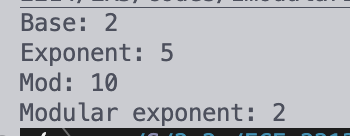
\includegraphics[width=.8\linewidth, height = .73in]{images/output/expo1.png}
        \caption*{}
        \label{fig:expo1}
    \end{subfigure}
    \begin{subfigure}{.5\textwidth}
        \centering
        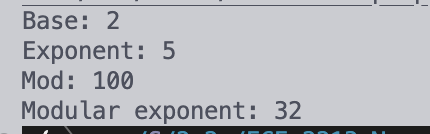
\includegraphics[width=.8\linewidth]{images/output/expo2.png}
        \caption*{}
        \label{fig:expo2}
    \end{subfigure}
    \begin{subfigure}{.5\textwidth}
        \centering
        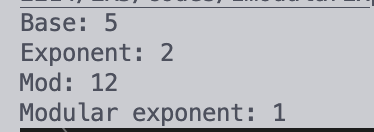
\includegraphics[width=.8\linewidth]{images/output/expo3.png}
        \caption*{}
        \label{fig:expo3}
    \end{subfigure}
    \begin{subfigure}{.5\textwidth}
        \centering
        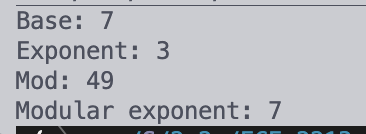
\includegraphics[width=.8\linewidth]{images/output/expo4.png}
        \caption*{}
        \label{fig:expo4}
    \end{subfigure}
    \caption{Outputs for Modular Exponentiation}
    \label{fig:expo}
\end{figure}
\begin{figure}[H]
    \begin{subfigure}{.5\textwidth}
        \centering
        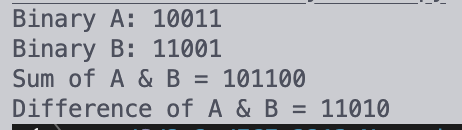
\includegraphics[width=.8\linewidth]{images/output/bin1.png}
        \caption*{}
        \label{fig:bin1}
    \end{subfigure}
    \begin{subfigure}{.5\textwidth}
        \centering
        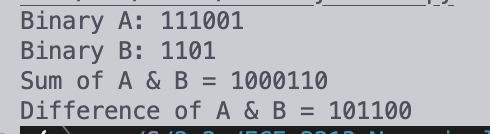
\includegraphics[width=.8\linewidth]{images/output/bin2.png}
        \caption*{}
        \label{fig:bin2}
    \end{subfigure}
    \newline
    \begin{subfigure}{.5\textwidth}
        \centering
        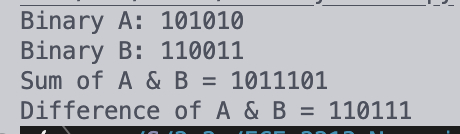
\includegraphics[width=.8\linewidth]{images/output/bin3.png}
        \caption*{}
        \label{fig:bin3}
    \end{subfigure}
    \begin{subfigure}{.5\textwidth}
        \centering
        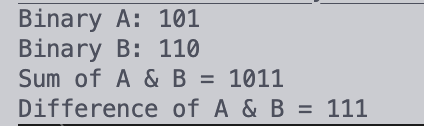
\includegraphics[width=.8\linewidth]{images/output/bin4.png}
        \caption*{}
        \label{fig:bin4}
    \end{subfigure}
    \caption{Outputs for Contraposition}
    \label{fig:bin}
\end{figure}

\begin{figure}[H]
    \begin{subfigure}{.5\textwidth}
        \centering
        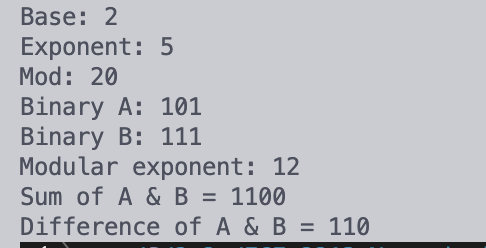
\includegraphics[width=.8\linewidth]{images/output/int1.png}
        \caption*{}
        \label{fig:int1}
    \end{subfigure}
    \begin{subfigure}{.5\textwidth}
        \centering
        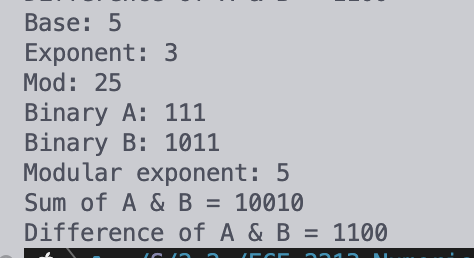
\includegraphics[width=.8\linewidth, height=1.1in]{images/output/int2.png}
        \caption*{}
        \label{fig:int2}
    \end{subfigure}
    \begin{subfigure}{.5\textwidth}
        \centering
        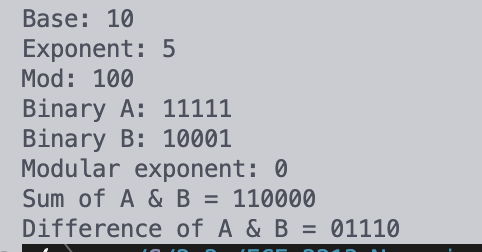
\includegraphics[width=.8\linewidth,]{images/output/int3.png}
        \caption*{}
        \label{fig:int3}
    \end{subfigure}
    \begin{subfigure}{.5\textwidth}
        \centering
        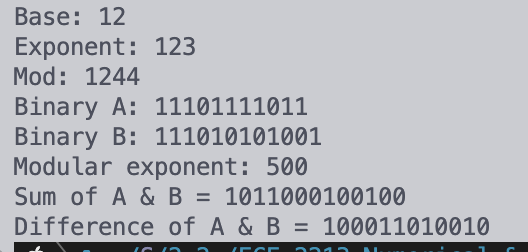
\includegraphics[width=.8\linewidth]{images/output/int4.png}
        \caption*{}
        \label{fig:int4}
    \end{subfigure}
    \caption{Outputs for Logical Equivalence}
    \label{fig:int}
\end{figure}


\section*{Analysis}
\subsubsection*{Code explanation}
The above code is only for finding an expression's tautology if the expression has only two variables and if the expression only contains AND, OR, NOT logics. The two variables can be the same, but for more than two variables, the code will not work.
In the code, first an input, the logical expression is taken. Then the spaces in that expression is removed, and then the variables are stored in separate variables. Then using a function, the variables are assigned their boolean values with all possible combinations, and evaluated using another function. At the same time, the truth table of the expression is printed.
Here, an integer variable $cnt$ is kept, initialized as $0$, whenever a case is false, it increments the variable. Finally, if $cnt > 0$, the expression is evaluated as $Not\ tautology$. Otherwise, the expression will be evaluated as $Is\ tautology$.

\section*{Discussion}
The code is only applicable for simple two variable logical expression. It's not efficient either. There are many other ways it can be done. Due to lack of knowledge, it was not possible for me to do it.
\\If the code was efficient and more usable for versatile expression, this experiment would've been more successful. For now, the code is satiable.

\bibliographystyle{IEEEtran}
\bibliography{ref}

\end{document}